\chapter{Agent Design}
In this chapter the agents' gameplay strategy will be described as well as its architecture and implementation design.

TODO Intro.

\section{Agent Strategy}
Before any strategies for mid-game or late-game could be devised, the bot must first master early-game. If the bot loses in early-game, the match will never proceed to later stages. Compared to matches between humans, the game usually ends much quicker, rarely leaving early-game. This is because later stages of the game involves many more kinds of units and strategies, such that the AI must be more advanced. Therefore, it seems prudent to first perfect the early game of the bot. From there, if time allows, the bot could attempt mid-game tactics.

Simplest solution is implementing one strategy, which can be expanded into mid-game if the round drags on that long. Both boom and turtle strategies seek to push the match out of early game, so the remaining strategy which lies in early game is rush. This has seen a lot of use in the bot tournaments, probably being the most popular choice. It requires nothing but building the earliest combat unit and attacking. When moving on to mid-game, additions could include upgrading, expanding to new resources or moving on to more advanced units. Even a failed rush would put pressure on the opponent, allowing the bot to compete in later stages of the match. This makes such a strategy sustainable in case the bot reaches mid-game, but is also proven to be a strong early-game strategy.

The bot will only focus on a single race. Even though Protoss are the slowest of the three, they also have the strongest and easiest to use early troops. This makes it a strong rush candidate, as it can easily beat opposing races' rushes if prepared. While the main AI challenges between races are shared, gameplay elements differ quite a lot.

\section{Architecture Design}
The imperative when designing the bot is to lessen the decision space as greatly as possible. The problems the bot faces are easily divided into smaller, isolated problems. Its therefore possible to construct the bot out of individual \emph{modules}, each solving some subset of problems. This isolation lessens the amount of concurrent decisions and information available to the agent, reducing the decision space.

These modules are structured in a \emph{hierarchy}. A superior module can command a subordinate, however only in terms of a \emph{black box}, without knowledge of its internal structure. By limiting the information available to the superior, we can easily limit the decision space with clever design. The clear benefit of this structure is easy replacement of individual modules, without damaging or refactoring neighbors. On the other hand, modules will inherently be limited with information, but we must trust that not all available data is required or even relevant for all decisions.

The UAlberta bot by Dave Churchill uses such a module structure, however it places them in an interesting hierarchy. The modules in the bot are in a \emph{arborescence} graph structure, that is, there is a root module which has exactly one path to each other node in the hierarchy. In other words there are no cyclic dependencies, and it is related to a tree structure, except a single module can have multiple parents. Churchill alleges that it is based on "proven military structures" - in any case the UAlberta bot is high-ranking bot, victor of one competition and runner up in others. The data-structure must have been proven to work by now.

The benefits of this structure is lesser and easier dependencies, removing the inherent challenges in cyclic dependencies. It enhances the benefits of modular design, since modules has a stricter position in the hierarchy, making the modular design easier. It is also a great boon to agile development, as the tree will simply evolve upwards with newer modules as superiors to the older. The lower modules make smaller decisions with fewer resource such as building and gathering, and the higher modules control more information to make the larger scale decisions such as strategies and attacking.

On the other hand, the structure allows less complicated interactions. By limiting the hierarchy, the information available is limited as some modules must be at the bottom of the hierarchy. These are inevitably void of interactions with higher modules. This is also felt at the root of the structure, as at some point all the choices have to be made in the final module. Figure \ref{fig:hierarchy} depicts the hierarchy structure, where higher modules are dependent on lower modules.

\begin{figure}
	\centering
	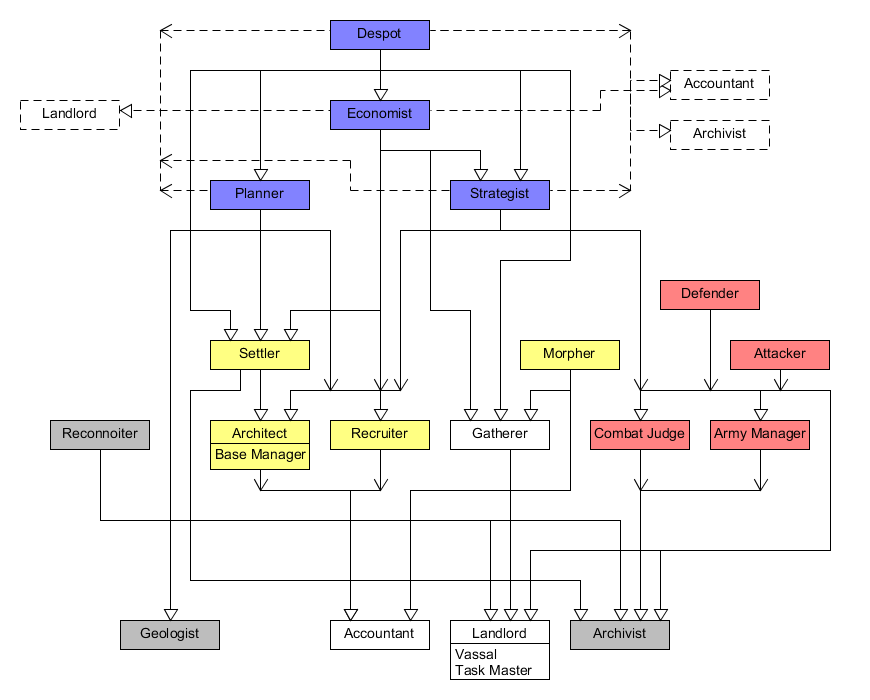
\includegraphics[width=\textwidth]{figures/Hierarchy}
\caption{Diagram of the module hierarchy}
\label{fig:hierarchy}
\end{figure}

%TODO Hierarchy diagram + description.

In the following chapters, we will describe the different groups of modules in the hierarchy and the problems they solve. While the modules are individually separate, some clusters of them are also separate. These can be separated in chapters as few of the modules has any connections between. The order of clusters is bottom-up so as to follow the chain of command. These groups are \emph{resources}, \emph{production}, \emph{information}, \emph{combat} and \emph{strategy}.

The following chapters cover the different groups of modules. They are:
\begin{itemize}
	\item Chapter \ref{ch:resources}
	\item Chapter \ref{ch:production}
	\item Chapter \ref{ch:exploration}
	\item Chapter \ref{ch:combat}
	\item Chapter \ref{ch:strategy}
\end{itemize}

Finally, Chapter \ref{ch:results} presents and discusses the results of the bot and the project as a whole.

	\subsection{Implementation}
	%Tidligt i rapporten, evt. som underafsnit til Agent Design. Her ville afsnittet primært handle meget overordnet kode-stil og om hvordan officer-systemet er implementeret:
	%- Er der brugt interfacet, templates eller andet finurligt?
	%- Hvordan snakker du med BWAPI? Problemer? Løsninger?
	%- Hvordan fungerer informations-udveksling mellem officererne?
	%- Hvordan fungerer kommando-mekanikker: direkte funktionskald, push "kommandoer" på en kø til senere inspektion, sæt et flag, osv?
	%- Var dine løsninger til ovenstående ad-hoc, løbende revurderet eller fra starten af grundigt og systematisk indtænkt?
		
	%Derudover kunne du have en kort beskrivelse af din generelle brug af C++
	%- C++11 eller ældre?
	%- Bruger du STL til data strukturer?
	%- Har du fulgt nogle særlige konventioner?
	%- Har du med vilje undgået visse subsets af C++? (dette er normalt fordi C++ er et lidt sygt sprog) Hvorfor?
	%- Er din kode systematisk kommenteret? Hvordan?
	%- Hvor mange kilde-filder har du og hvor mange linjer kode er der i alt?